\documentclass[twocolumn]{article}
\linespread{1.1}
\usepackage{charter}
\usepackage{booktabs}
\usepackage{xcolor}
\usepackage{graphicx}
\usepackage[switch]{lineno}
\renewcommand\linenumberfont{\normalfont\tiny\sffamily\color{blue}}
\linenumbers
\usepackage{flushend}
\usepackage{blindtext}
\usepackage{hyperref}
\begin{document}
\title{Project Report Template}
\author{Sayed Hadi Hashemi, Roy H. Campbell \\ \small University of Illinois at Urbana-Champaign}
\date{}
\maketitle
\section{Introduction}
% Remove Me
  \blindtext[3]

  % Sample Figure  
  As shown in figure~\ref{fig:sample}.

  \begin{figure}[tbh]
    \centering
    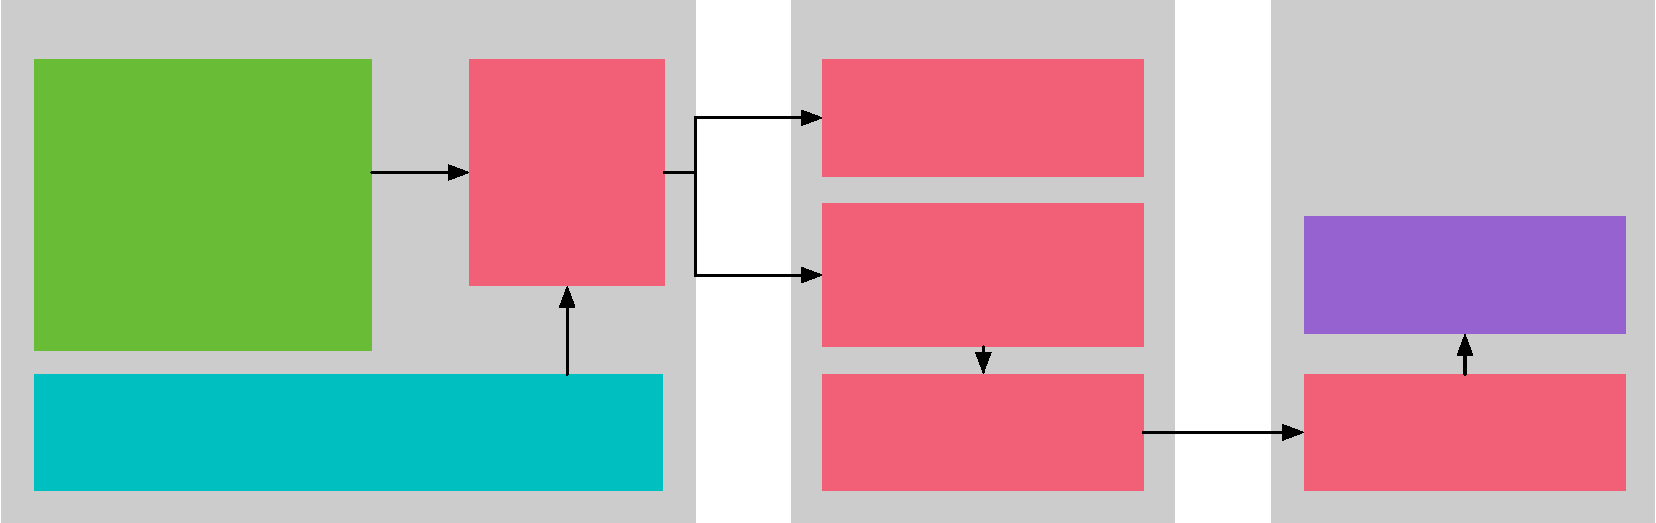
\includegraphics[width=\columnwidth]{sample-figure.pdf}
    \label{fig:sample}
    \caption{Sample Architecture}
  \end{figure}
  
  \blindtext[3]

  % Sample Table
  As shown in table~\ref{table:sample}.
  
  \begin{table}
  \centering
  \begin{tabular}{@{}ccc@{}}
  \toprule
  Nodes & Speed up & Overhead\\
  \midrule
  8 & 2.1 & 11\\
  64 & 4.5 & 29 \\
  \bottomrule
  \end{tabular}
  \label{table:sample}  
  \caption{Sample Table}
  \end{table}


\section{Related Work}
% Remove Me
  \blindtext
  % Sample Citation
  \cite{Hashemi2018}
  \blindtext[3]
  \blindtext[3]

{\footnotesize 
\bibliographystyle{acm2}
\bibliography{references.bib}}
\end{document}
